\begin{solution}
The minimum time  for all dogs to pass the bridge is 24 minutes.\\[0.2cm]

Let us number the dogs by their weight. In the first stage, dogs number 1, 2 and 4 cross the bridge (4 minutes). In the second step, dog 1 will return (1 minute). In the third stage, dogs 6 and 8 cross the bridge (8 minutes).
\begin{center}
	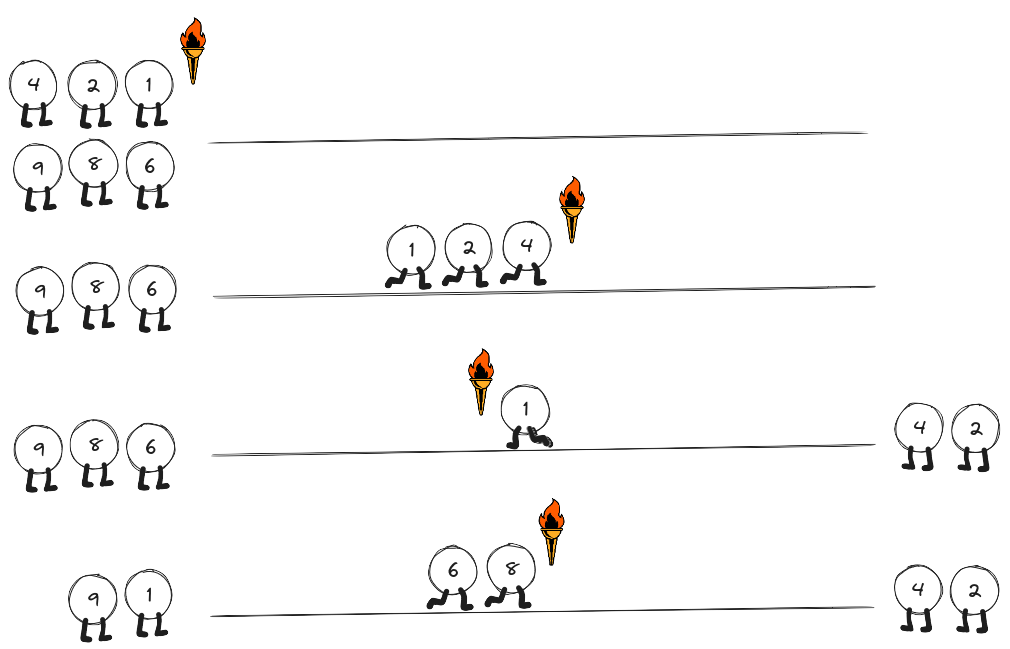
\includegraphics[width=9cm]{40/figs/40_diagram0.png}
\end{center}

In the fourth stage, dog 2 returns (2 minutes). And finally, in the fifth stage, dogs 1, 2 and 9 will pass the bridge (9 minutes).

\begin{center}
	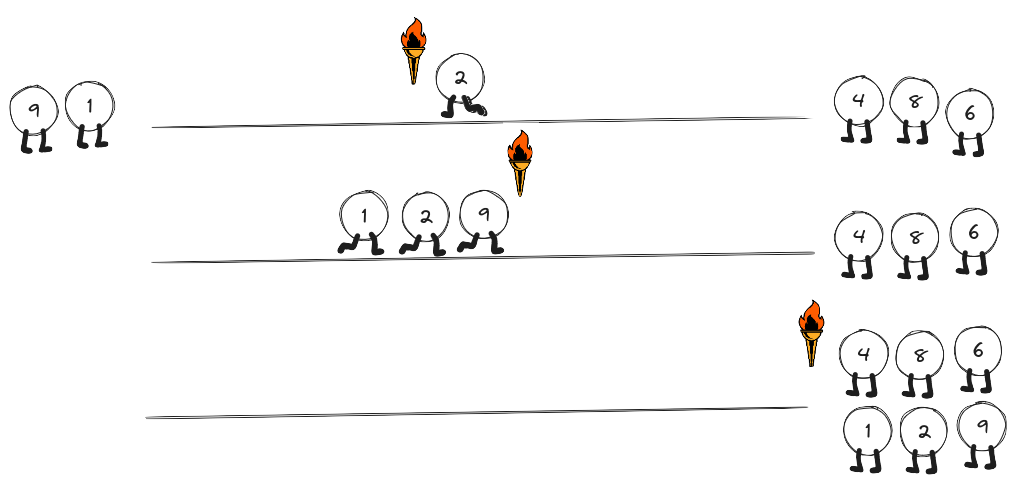
\includegraphics[width=9cm]{40/figs/40_diagram1.png}
\end{center}

The total amount of time for all dogs to cross the bridge is equal to $4+1+8+2+9 = 24$ minutes.
\end{solution}